\newpage
\section{Design pattern}
\subsection{Iterator}

\subsubsection{Explication générale}

Tout d'abord, la "classe" musique présente sur le diagramme n'existe pas vraiment, mais nous avons décidé de la représenter quand même pour faciliter la compréhension. Cette "classe" représente juste le chemin d'accès, en String, à une musique.
Au lancement du jeu, un objet MusicGestion va être instancié.
Lors de cette instanciation, nous allons créer une liste de String, ces String sont des chemins d'accès relatif pour pouvoir accéder aux différentes musiques du jeu.
Nous allons ensuite instancier un objet IteratorMusic qui prendra en paramètre cette liste.
Dans la méthode gererMusic, nous allons appeler la méthode item() de la classe IteratorMusic.
Cette méthode nous permet de renvoyer l'objet sur lequel nous sommes actuellement en train d'interagir.
Ensuite, la méthode gererThread va être appelée, cette méthode va faire appel à la méthode next() de la classe IteratorMusic.
Celle-ci va permettre d'accéder à l'objet suivant dans la liste de l'itérator.
La méthode gererMusic sera de nouveau appeler permettant ainsi d'avoir la musique suivante.
Dans le cas où la liste de l'itérator a été entièrement parcourue, une condition, présente dans la méthode item() de la classe IteratorMusic, va appeler la méthode reset() présente dans cette même classe.
Cette méthode permet de revenir directement au début de la liste, pour ainsi boucler sur celle-ci.


\subsubsection{Diagramme de classe}

\begin{figure}[h]
	\centering
	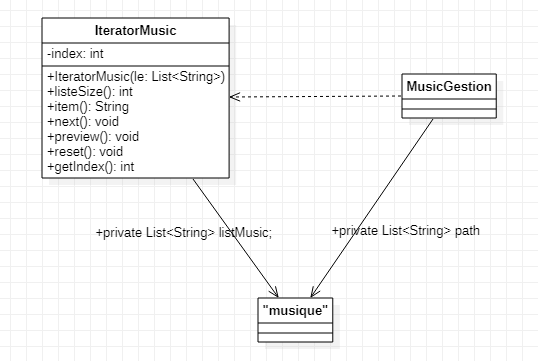
\includegraphics[width=\textwidth]{ttmc_iterator.png}
	\caption{Diagramme de l'iterator}
	\label{fig:diag_iterator}
\end{figure}

\subsubsection{Extrait de code source}
\lstinputlisting[language=Java]{IteratorMusic.java}

\newpage
\subsection{Template Method}

\subsubsection{Explication générale}

Notre objectif était de rendre notre programme plus accéssible aux gens que ne parlent pas l'anglais. Appliquer un concept d'internationalisation était alors notre objectif. Étant donné que l'on savait que le résultat obtenu ne se baserait que sur la langue chosie par l'utilisateur, le simple fait de savoir que les manipulations seraient exactement les mêmes, on a donc décidé de mettre en place le Design Pattern: Template Method. Voici le mécanisme:
\begin{enumerate}
\item Le programme detecte la langue choisie par l'utilisateur, si aucune langue a été choisie, alors le programme créera une nouvelle instance de English, soit, il mettra le jeu en anglais par défaut.
\item Lors de l'instanciation des boutons ou différentes messages textuels, la fonction getString qui renverra la chaîne de caractère propre à ce dernier traduite dans la langue choisie.
\end{enumerate}

Si l'utilisateur choisi une langue différente, alors le programme fera une appel à la classe qui corréspond à la langue.
Les différents cas possibles sont:
\begin{itemize}
\item English() pour l'anglais
\item French() pour le français
\item Italian() pour l'italien
\item Japanese() pour le japonais
\end{itemize}

\subsubsection{Diagramme de classe}

\begin{figure}[h]
	\centering
	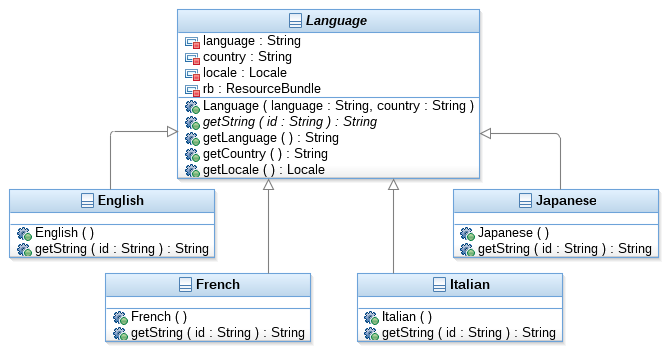
\includegraphics[width=\textwidth]{ttmc_template_method.png}
	\caption{Diagramme du template method}
	\label{fig:diag_template_method}
\end{figure}

\subsubsection{Extrait de code source}
Voici l'histoire d'un nain capable de courir vite et de voyager loin.\\
Dans son épopée formidable nous le suivrons une bière à la main.\\
\lstinputlisting[language=Java]{Language.java}

